%%%%%%%%%%%%%%%%%%%%%%%%%%%%%%%%%%%%%%%%%%%%%%%%%%%%%%%%%%%
%                                                         %
% CHAPTER 02:                                             %
% Theoretical basis of the simulation                     %
%                                                         %
% This file is part of a BSc Thesis Project. See the      %
% LICENSE file for more information about licensing.      %
%                                                         %
% Author:     Matteo Seclì <secli.matteo@gmail.com>       %
% A.Y.:       2014/2015                                   %
% URL:        https://github.com/matteosecli/QMC          %
%                                                         %
%%%%%%%%%%%%%%%%%%%%%%%%%%%%%%%%%%%%%%%%%%%%%%%%%%%%%%%%%%%

\graphicspath{{Mainmatter/figures/PNG/}{Mainmatter/figures/PDF/}{Mainmatter/figures/}}

\chapter{Theoretical basis of the simulation}

\section{The Variational Principle}
The Variational Principle is a method of general validity that can be used to gather information about a system with a Hamiltonian that we are unable to diagonalize (i.e., we can't solve the Schr\"{o}dinger equation for that system). Specifically, this principle gives us an \emph{upper bound} for the energy of the ground state, that we will call here $E_{\text{gs}}$. The formulation is astonishingly simple: if you pick \emph{any state $\Ket{\psi}$ whatsoever}, then
\begin{equation}
	E_{\text{gs}} \leq \frac{\Braket{\psi|\hat{H}|\psi}}{\Braket{\psi|\psi}}.
	\label{eq:variational_equation}
\end{equation}
In this project we are going to use just this formula, because you see that the normalization of the state is not necessary. But if you have a normalized state, then equation (\ref{eq:variational_equation}) is further simplified in
\begin{equation}
	E_{\text{gs}} \leq \Braket{\psi|\hat{H}|\psi} \equiv \Braket{\hat{H}}.
\end{equation}

This equation seems a kind of magic but actually the proof of this fact is really simple, and we are going to sketch here a proof to show the power of this method (roughly, as it appears in \cite{Griffiths2005}).
\begin{proof}
	Since the (unknown) eigenstates $\Ket{\psi_n}$ of $\hat{H}$ form a complete set, we can expand our random state $\Ket{\psi}$ on this basis:
	\begin{equation*}
		\Ket{\psi} = \sum_{n} C_n\Ket{\psi_n},
		\qquad
		C_n \in \mathbb{C},
	\end{equation*}
	where the $\Ket{\psi_n}$'s are such that
	\begin{equation*}
		\hat{H}\Ket{\psi_n} = E_n\Ket{\psi_n}.
	\end{equation*}
	Then, we have
	\begin{align*}
		\Braket{\psi|\hat{H}|\psi}
		&= \sum_{nm} C_m^* C_n E_n \underbrace{\Braket{\psi_m|\psi_n}}_{\delta_{mn}} \\
		&= \sum_{n} |C_n|^2 E_n, \\
		\Braket{\psi|\psi}
		&= \sum_{n} |C_n|^2.
	\end{align*}
	Since $E_n \geq E_{\text{gs}} \; \forall n$, it follows immediately that
	\begin{equation}
		E_T 
		\doteqdot \frac{\Braket{\psi|\hat{H}|\psi}}{\Braket{\psi|\psi}}
		= \frac{\sum_{n} |C_n|^2 E_n}{\sum_{n} |C_n|^2}
		\geq \frac{\cancel{\sum_{n} |C_n|^2} E_{\text{gs}}}{\cancel{\sum_{n} |C_n|^2}}
		= E_{\text{gs}}.
		\label{eq:var_princ_end_proof}
	\end{equation}
\end{proof}

In practice, one chooses a class of states for $\Ket{\psi}$ parametrized by one or more parameters -- the so-called \emph{variational parameters}, and then calculates the quantity $E_T$ for multiple sets of values of the variational parameters $\alpha_1\ldots,\alpha_n$. The lower value of $E_T$ obtained in this way is the required upper bound. If one manages to find an even lower value for $E_T$ with a more clever wave-function, then he has found a better upper bound for the ground state energy.

The only trouble with this method is that we never know for sure how close we are to the \emph{actual} ground state energy; all we get for sure is just an upper bound. However, if one manages to guess a \emph{realistic} $\Ket{\psi}$, he often gets values for the ground state energy that miraculously match the actual ones.

In the following, we represent $\Ket{\psi}$ in its function-representation as
\begin{equation*}
	\Ket{\psi} \simeq \psi_T,
\end{equation*}
where ``$\simeq$'' means ``represented by'' and the subscript $T$ is just to remember that $\psi_T$ is our \emph{trial} wave-function.

In our case the Hamiltonian lies in an infinite-dimension Hilbert space, so we have to replace the sums in (\ref{eq:var_princ_end_proof}) with integrals over all the space. Indicating with $d\vec{\tau}$ a space element, we can write
\begin{equation}
	E_T = \frac{\int d\vec{\tau} \, \psi_T^* \hat{H} \psi_T}{\int d\vec{\tau} \, |\psi_T|^2}.
	\label{eq:var_energy_integral}
\end{equation}

Calculating $E_T$ as it appears in (\ref{eq:var_energy_integral}) is not a piece of cake. However, we can recast that equation in a simpler form if we multiply and divide by $\psi_T$ at the left of $\hat{H}$. In fact,
\begin{align}
	E_T 
	&= \frac{\int d\vec{\tau} \, \psi_T^* \dfrac{\psi_T}{\psi_T} \hat{H} \psi_T}{\int d\vec{\tau} \, |\psi_T|^2} \\
	&= \frac{\int d\vec{\tau} \, |\psi_T|^2 \dfrac{1}{\psi_T} \hat{H} \psi_T}{\int d\vec{\tau} \, |\psi_T|^2} \\
	&= \int d\vec{\tau} \, \frac{|\psi_T|^2}{\int d\vec{\tau} \, |\psi_T|^2} \frac{1}{\psi_T} \hat{H} \psi_T \\
	&= \int d\vec{\tau} \, \mathcal{P}(\vec{\tau}) E_L(\vec{\tau}) \\
	&\simeq \frac{1}{n} \sum_{i = 1}^{n} E_L(\vec{\tau})
\end{align}
where
\begin{equation}
	\mathcal{P}(\vec{\tau}) = \frac{|\psi_T|^2}{\int d\vec{\tau} \, |\psi_T|^2}
\end{equation}
and
\begin{equation}
	E_L(\vec{\tau}) = \frac{1}{\psi_T} \hat{H} \psi_T.
\end{equation}
The dependence of $\psi_T$ on the position in space and on the variational parameters has been omitted just for better readability. The quantity $E_L$ is called the \emph{local energy}, and it's what we are going to calculate in this project. Obviously, for bigger $n$ we obtain better results.

\section{Considerations about the physical system}
\label{sec:considerations}
Our system is represented by a number $N$ of electrons that have total energy
\footnote{
Calling the Hamiltonian the total energy is improper. Rather it should be called the \emph{generalized energy}, since in general it is \emph{not} the total energy because it also contains terms of the 1st and 0th order in the generalized velocities. However in this case the system does not contain non-conservative forces (from which the extra terms stem), so we can safely identify the Hamiltonian with the total energy.
}
\begin{equation}
	\hat{H} = 
	\sum_{i=1}^{N} \left( -\frac{1}{2}\nabla_i^2 + \frac{1}{2}\omega^2r_i^2 \right)
	+ \sum_{i<j}\frac{1}{r_{ij}},
	\label{eq:full_hamiltonian}
\end{equation}
where $r_{ij} = |\vec{r}_i - \vec{r_j}|$ and natural units $( \hbar = c = e = m_e = 1)$ are used in order to have the energy in atomic units. You see that the Hamiltonian includes a standard part (a harmonic oscillator) plus a repulsion potential, that is the one that gives troubles in analytical calculations.

An important feature of our system is that it is made up of \emph{identical particles}. Let's try to exploit this feature to simplify our trial wave-function.

Suppose that we have a system made up of two particles, let's call them 1 and 2. Then, the state $\Ket{\psi}$ of the system can be expressed (for example) as
\begin{equation}
	\Ket{\psi} = \Ket{1} \otimes \Ket{2}.
\end{equation}
Now we can introduce the \emph{permutation operator} $\hat{P}$, defined as
\begin{equation}
	\hat{P} \Ket{1} \otimes \Ket{2} \doteqdot \Ket{2} \otimes \Ket{1}.
\end{equation}
One immediately sees that $\hat{P} = \hat{P}^{\dagger}$ and $\hat{P}^2 = \hat{I}$ ($\hat{I}$ is the identity operator), which means that $\hat{P}$ is hermitian and unitary. These two properties allow us to say that the eigenvalues of $\hat{P}$ are $\pm 1$. In general, this operator $\hat{P}$ does not commute with $\hat{H}$; but -- and here is the trick -- it \emph{does} commute with $\hat{H}$ for a system of \emph{identical particles}. Since in that case $[\hat{H},\hat{P}] = 0$, the eigenstates of $\hat{H}$ must also be eigenstates of $\hat{P}$. Recalling that the eigenvalue of $\hat{P}$ are $\pm 1$, one can rewrite the state $\psi$ as
\begin{equation}
	\Ket{\psi} = \frac{1}{\sqrt{2}} \Big( \Ket{1} \otimes \Ket{2} \pm \Ket{2} \otimes \Ket{1} \Big)
	\label{eq:identical_particles}
\end{equation}
to make it also eigenstate of $\hat{P}$. You see that, in this form, the state is either symmetric or antisymmetric; particles with symmetric wave-function are called \emph{bosons}, and particles with antisymmetric wave-function are called \emph{fermions}. It turns out that electrons are fermions, so we are interested only in the antisymmetric case. Rewriting the fermions wave-function in coordinate representation, we obtain:
\begin{align}
	\psi(\vec{r}_1,\vec{r}_2,\sigma_1,\sigma_2) 
	&= \Big( \Bra{\vec{r}_1} \otimes \Bra{\vec{r}_2} \Big) \Ket{\psi}
	= \frac{1}{\sqrt{2}} \Big( \Braket{\vec{r}_1|1}\Braket{\vec{r}_2|2} - \Braket{\vec{r}_1|2}\Braket{\vec{r}_2|1} \Big) \\
	&= \frac{1}{\sqrt{2}} \Big( \phi_1(\vec{r}_1,\sigma_1)\phi_2(\vec{r}_2,\sigma_2) - \phi_2(\vec{r}_1,\sigma_2)\phi_1(\vec{r}_2,\sigma_1) \Big)
	= \frac{1}{\sqrt{2}} \left\lvert
	\begin{array}{cc}
		\phi_1(\vec{r}_1,\sigma_1) & \phi_1(\vec{r}_2,\sigma_1) \\
		\phi_2(\vec{r}_1,\sigma_2) & \phi_2(\vec{r}_2,\sigma_2)
	\end{array}
	\right\lvert
	\label{eq:slater_example}
\end{align}
where the $\phi_i$'s are the single-particle wave-functions, the $\sigma_i$'s just indicate the explicit dependence on the spin, and the determinant in (\ref{eq:slater_example}) is called the \emph{Slater determinant}. For $N$ particles the determinant has exactly the same shape (is just a $N \times N$ matrix) and the factor $\frac{1}{\sqrt{2}}$ is replaced with $\frac{1}{\sqrt{N!}}$. However, we don't care about the normalization factor because it's not required to apply the variational principle.

We can recast this equation in a simpler form. In fact, it's possible to rewrite $\Ket{\phi}$ as
\begin{equation}
	\Ket{\phi} = \Ket{\eta} \otimes \Ket{\chi},
\end{equation}
where $\Ket{\eta}$ is the \emph{spatial part} and $\Ket{\chi}$ is the \emph{spin part}. Note that -- since the Hamiltonian is spin-independent -- the spin part just takes into account the spin configuration of the system, and it has nothing to do with the positions of the particles themselves! In other words, while the spatial part depends on the positions of the particles, the spin part does not at all and we can ``forget'' about it if we are smart. 

In fact, the best way to minimize the energy is to put the two electrons in the same orbital. This means that the spatial part is \emph{symmetric} under the interchange of two particles; but we have also said that this wave-function has to be antisymmetric. So, the spin part has to be \emph{antisymmetric}. If you look at the Clebsch-Gordan table for combining two spin-1/2 (Figure \ref{fig:CGt}), you see that the only antisymmetric combination is the total spin state $\Ket{0,0}$, that can be written as
\begin{equation}
	\Ket{0,0} 
	= \frac{1}{\sqrt{2}}
	 \left( \Ket{\uparrow} \otimes \Ket{\downarrow} 
	- \Ket{\downarrow} \otimes \Ket{\uparrow} \right)
	\label{eq:total_spin}
\end{equation}

This fact permits a simplification of the Slater determinant; in fact, if we suppose -- for example --  that particle $1$ has spin-up and particle $2$ has spin-down, we can write
\begin{equation}
	\Psi_T(\vec{r}_1,\vec{r}_2,\sigma_1,\sigma_2) 
	=\left\lvert
	\begin{array}{cc}
		\phi_1(\vec{r}_1,\sigma_1) & \phi_1(\vec{r}_2,\sigma_1) \\
		\phi_2(\vec{r}_1,\sigma_2) & \phi_2(\vec{r}_2,\sigma_2)
	\end{array}
	\right\lvert
	= \phi_1(\vec{r}_1)\phi_2(\vec{r}_2).
\end{equation}
where the $\phi_i$'s are now independent on the spin. In other words, they are just the spatial parts $\eta_i$'s of the single-particle wave-functions. You also see that, since now the single-particle wave-functions are independent on the spin, the are \emph{exactly} the same function because they occupy the same energy level!

The generalization to $N$ particles is straightforward, and will be given later.

\begin{figure}[H]
	\centering
	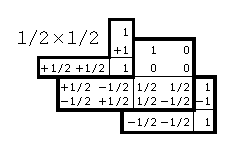
\includegraphics[width=0.28\textwidth]{CGt}
	\caption{The Clebsch-Gordan table for combining two spin-1/2. Source: \url{http://pdg.lbl.gov/2002/clebrpp.pdf}.}
	\label{fig:CGt}
\end{figure}

\section{The Metropolis algorithm}

Let's first briefly introduce what a \emph{Markov chain} is. We call a Markov chain a stochastic process where the transition probability that characterizes the transition between states only depends on the previous step and not from the path to get to such step. We can then write \citep[see][]{Hjorth-Jensen2014}
\begin{equation}
	w_i(t+\delta t)=\sum_i W(j \rightarrow i) w_j (t),
	\label{eq:markov_definition}
\end{equation}
where $w_i(t+\delta t)$ is our PDF -- in our case $|\psi_T(R)|^2$ and $W(j \rightarrow i)$ is the probability of jumping from $j$ to $i$, also called the \emph{transition probability}. We also have
\begin{equation}
	\sum_{i}w_i(t) = 1.
\end{equation}
due to the normalization condition. We can see from equation (\ref{eq:markov_definition}) the probability density function at $t+\delta t$ only depends on its previous state $t$. 

In the case of infinite dimensionality, representing $W$ as a matrix, we have
\begin{equation}
	\hat{w}(t+\delta t) = \hat{W}\hat{w}(t).
\end{equation}
from which
\begin{equation}
	\hat{w}(\infty)= \hat{W} \hat{w}(\infty).
\end{equation}
Then, the problem is just an eigenvalue problem with eigenvalue $1$.

Now, let's consider an \emph{ergodic} system, where the average over time of a process is the same as the ensemble average. Or in other words, as one increases the steps, there exists a positive probability measurement at step $n$ that is independent on the probability distribution at the initial step $0$. It holds
\begin{equation}
	W(i \rightarrow j) w_i= W(j \rightarrow i) w_j,
\end{equation}
from which
\begin{equation}
	R \doteqdot \frac{W(i \rightarrow j)}{W(j \rightarrow i)}=\frac{w_j}{w_i}=\frac{|\psi_T (r^{\text{new}})|}{|\psi_T (r^{\text{old}})|}.
\end{equation}

Since $W(i \rightarrow j)$ is unknown, we model it as the product of two probabilities:
\begin{equation}
	W(i \rightarrow j)=A(i \rightarrow j) \, T(i \rightarrow j),
\end{equation}
where $A(i \rightarrow j)$ is the probability of accepting the move and $T(i \rightarrow j)$ is the probability to transition from the state $i$ to the state $j$. In a similar way we can write:
\begin{equation}
	W(j \rightarrow i)=A(j \rightarrow i) \, T(j \rightarrow i).
\end{equation}

\subsection{Brute force sampling}
The \emph{brute force} Metropolis algorithm simply consists in the assumption that the transition probability is symmetric, that is
\begin{equation}
	T(i \rightarrow j)= T (j \rightarrow i),
\end{equation}
which leads to
\begin{equation}
	\frac{W(i \rightarrow j )}{W(j \rightarrow i)}=\frac{A(i \rightarrow j )}{A(j \rightarrow i)}.
\end{equation}
Then, we can distinguish between two cases.
\begin{itemize}
	\item If $\dfrac{w_j}{w_i}\geq 1$, then
	\begin{equation}
		A(i \rightarrow j ) \geq A(j \rightarrow i).
	\end{equation}
	So, if we manage to move to such a state, we accept this move because we are moving to a higher probability region.
	\item If $\dfrac{w_j}{w_i} < 1$, then
	\begin{equation}
		A(j \rightarrow i ) > A(i \rightarrow j).
	\end{equation}
	We can't blindly reject this move just because we are moving to a lower probability region, but we can't also accept all of this kind of moves. So, what one does is to compute a random number $r \in (0,1)$ and to accept the move if $r \leq w_j/w_i$.
\end{itemize}
To summarize, one sets
\begin{equation}
	A(i\rightarrow j) 
	= \text{min} \left(1, \frac{w_j}{w_i} \right)
	= \text{min} \left(1, \frac{|\psi_T(r^{\text{new}})|^2}{|\psi_T(r^{\text{old}})|^2} \right)
\end{equation}
and then compares with a random number $r \in (0,1)$. If $A(i\rightarrow j) \geq r$ the step is accepted, otherwise it's rejected.

\subsection{Importance sampling and Schödinger equation as a diffusion problem}
\label{sec:importance}

\emph{Importance sampling} consists in doing more clever assumptions on the shape of $T(i \rightarrow j)$. The discussion is the same as the brute force case, but this time we have to set
\begin{equation}
	A(i\rightarrow j) 
	= \text{min} \left(1, \frac{w_jT(j \rightarrow i)}{w_iT(i \rightarrow j)} \right)
	= \text{min} \left(1, \frac{|\psi_T(r^{\text{new}})|^2T(j \rightarrow i)}{|\psi_T(r^{\text{old}})|^2T(i \rightarrow j)} \right).
	\label{eq:acceptance_imp}
\end{equation}
If we recast the Schr\"{o}dinger equation as a diffusion problem, $T(i \rightarrow j)$ is going to be a Gaussian distribution (or a modified Gaussian); let's do that.

The main idea is to model $T(i \rightarrow j)$ in order to reflect the shape of the trial wave-function itself and have in this way a more ``intelligent'' walk, that wastes less points. The walk is generated using the Fokker-Planck and the Langevin equations; the former -- for a one-dimension diffusion problem -- is
\begin{equation}
	\frac{\partial P}{\partial t} = D \dfrac{\partial}{\partial x} \left( \dfrac{\partial}{\partial x} - F \right)P(x,t),
\end{equation}
where
$P(x,t)$ is the time-dependent probability density, $D$ is the \emph{diffusion coefficient} (it's $0.5$ for the Schr\"{o}dinger equation, see \cite{Hoegberget2013}) and $F$ is the \emph{drift term}.

The Langevin equation, on the other hand, reads as
\begin{equation}
	\frac{\partial x(t)}{\partial t} = DF(x(t)) + \eta,
	\label{eq:langevin}
\end{equation}
being $\eta$ a \emph{random variable}. By solving equation (\ref{eq:langevin}) with Euler's method, it follows that the new position is given by
\begin{equation}
	y = x + DF(x)\Delta t + \xi,
\end{equation}
being $\xi$ a \emph{Gaussian} random variable and $\Delta t$ a chosen time step.

For two or more dimensions, the Fokker-Planck equation is just
\begin{equation}
	\frac{\partial P}{\partial t} = \sum_i D \dfrac{\partial}{\partial \vec{x}_i} \left( \frac{\partial}{\partial \vec{x}_i} - \vec{F}_i \right)P(\vec{x}_i,t)
\end{equation}
We can obtain a convergence to a stationary probability density setting the left hand side to zero, that means all the terms of the sum must be equal to zero. Expanding the product, we obtain
\begin{equation}
	\frac{\partial^2 P}{\partial \vec{x}_i^2} = P \frac{\partial}{\partial \vec{x}_i}\vec{F}_i + \vec{F}_i \frac{\partial}{\partial \vec{x}_i}P.
\end{equation}
Since the drift vector has the form $\vec{F} = g(\vec{x}) \dfrac{\partial P}{\partial \vec{x}}$, we get
\begin{equation}
	\frac{\partial ^2 P}{\partial \vec{x}_i^2 } = P \frac{\partial g}{\partial P} \left( \frac{\partial P}{\partial \vec{x}_i} \right)^2 + Pg \frac{\partial ^2 P}{\partial \vec{x}_i^2} + g \left( \frac{\partial P}{\partial \vec{x}_i} \right)^2.
	\label{eq:intermediate_imp}
\end{equation}

If we want a stationary density the left hand side of equation (\ref{eq:intermediate_imp}) must be zero, and this is possible only if $g = \dfrac{1}{P}$. With this substitution, the drift vector reads as
\begin{equation}
	\vec{F} = \frac{1}{P} \nabla P.
	\label{eq:drift_vector}
\end{equation}
Since -- as we said many times before --  our probability density is the modulus squared of the trial wave-function, that is
\begin{equation}
	P = |\psi_T|^2,
\end{equation}
the drift vector in equation (\ref{eq:drift_vector}) finally reads as
\begin{equation}
	\vec{F} = 2 \frac{1}{\Psi_T} \nabla \Psi_T.
\end{equation}
Written in this way, $\vec{F}$ is also called the \emph{quantum force}. This force pushes the walker in those regions where the trial wave function is larger, increasing the efficiency of the simulation.

Solving the Fokker-Plank equation finally gives an expression for the transition probability $T(x \rightarrow y)$, that turns out can be expressed as the Green function
\begin{equation}
G(y,x, \Delta t) = \dfrac{1}{(4 \pi D \Delta t)^{3N/2}} \exp(-(y - x - D \Delta t F(x))^2 / 4 D \Delta t).
\end{equation}

With this expression, the acceptance ratio in equation (\ref{eq:acceptance_imp}) becomes
\begin{equation}
	R 
	= \frac{|\psi_T(y)|^2T(y \rightarrow x)}{|\psi_T(x)|^2T(x \rightarrow y)}
	= \frac{|\psi_T(y)|^2G(x,y,\Delta t)}{|\psi_T(x)|^2G(y,x,\Delta t)}.
\end{equation}


\subsection{Implementation}

\begin{figure}[H]
	\centering
	\begin{tikzpicture}[node distance=2cm]
	
		% Draw the nodes
		\node (start) [startstop, align=center] {Initialize:\\ Set $\vec{r}^{\text{old}}$, $\alpha$\\ and $\psi_{T-\alpha}(\vec{r}^{\text{old}})$};
		%\node (in1) [io, below of=start] {Input};
		\node (pro1) [process, below of=start] {Suggest a move};
		\node (pro2) [process, below of=pro1] {Compute\\ acceptance\\ ratio $R$};
		\node (dec1) [decision, below of=pro2, yshift=-0.5cm, align=center] {Is\\$R \geq r$?};
		\node (pro3a) [process, below of=dec1, yshift=-0.5cm, align=center] {Accept move:\\ $\vec{r}^{\text{old}} = \vec{r}^{\text{new}}$};
		\node (pro3b) [process, right of=dec1, xshift=2cm] {Reject move:\\ $\vec{r}^{\text{new}} = \vec{r}^{\text{old}}$};
		\node (dec2) [decision, below of=pro3a, yshift=-0.5cm, align=center] {Last\\ move?};
		\node (dec2left) [left of=dec2, xshift=-1cm] {};
		\node (pro5) [process, below of=dec2, yshift=-0.5cm] {Get local\\ energy $E_L$};
		\node (dec3) [decision, below of=pro5, yshift=-0.5cm, align=center] {Last\\ MC step?};
		\node (dec3left) [left of=dec3, xshift=-2cm] {};
		\node (pro6) [process, below of=dec3, yshift=-0.5cm, align=center] {Collect\\ samples};
%		\node (out1) [io, below of=pro2a] {Output};
		\node (stop) [startstop, below of=pro6] {End};
		
		%Draw the arrows
		\draw [arrow] (start) -- (pro1);
		\draw [arrow] (pro1) -- (pro2);
		\draw [arrow] (pro2) -- (dec1);
		\draw [arrow] (dec1) -- node[anchor=west] {yes} (pro3a);
		\draw [arrow] (dec1) -- node[anchor=south] {no} (pro3b);
		\draw [arrow] (pro3b) |- (dec2);
		\draw [arrow] (pro3a) -- (dec2);
		\draw [arrow] (dec2) -- node[anchor=west] {yes} (pro5);
		\draw [arrow] (dec2) -- node[anchor=south] {no} (dec2left.center) |- (pro1);
		\draw [arrow] (pro5) -- (dec3);
		\draw [arrow] (dec3) -- node[anchor=west] {yes} (pro6);
		\draw [arrow] (dec3) -- node[anchor=south] {no} (dec3left.center) |- (pro1);
		\draw [arrow] (pro6) -- (stop);
	
	\end{tikzpicture}
	\caption{Chart flow for the Quantum Variational Monte Carlo algorithm.}
	\label{fig:chart_flow}
\end{figure}

We can sum up the algorithm as follows. Given a random number generator that returns aleatory values in the interval $(0, 1)$ with a uniform (or Gaussian for the importance sampling) distribution, then the Metropolis algorithm consists in these steps.
\begin{itemize}
	\item Chosen a starting point $x_0$ and a step length $l$ (or a time-step $\Delta t$ for the importance sampling), a random number $\varepsilon$ is generated in the interval $(0, 1)$.
	\item The proposed step is $x^{\text{new}}=x^{\text{old}} + l\varepsilon$ (or $x^{\text{new}} = x^{\text{old}} + D\vec{F}(x^{\text{old}})\Delta t + \varepsilon$ for the importance sampling).
	\item The probability ratio $R = \frac{|\psi_T(r^{\text{new}})|^2T(j \rightarrow i)}{|\psi_T(r^{\text{old}})|^2T(i \rightarrow j)}$ is computed.
	\item A new random number $r$ is generated in the interval $(0, 1)$.
	\item If $R \geq r$, the step is accepted and the new position is stored by letting $x^{\text{old}}=x^{\text{new}}$.
	\item If $R < r$, the step is rejected and the new position is discarded by letting $x^{\text{new}}=x^{\text{old}}$.
\end{itemize}
A flow chart of this process is sketched in Figure \ref{fig:chart_flow}.